\documentclass[../main.tex]{subfiles}

\newcommand{\cdiff}{\text{c}_{\text{diff}}}
\newcommand{\cspec}{\text{c}_{\text{spec}}}
\newcommand{\clightcolor}{\text{c}_{\text{light}}}

\begin{document}
\chapter{Modele oświetlenia o podłożu fizycznym}

\section{Wstęp}

Ze względu na ograniczenia techniczne przez długie lata trójwymiarowe aplikacje czasu rzeczywistego nie mogły sprostać zadaniu wygenerowania wielu efektów świetlnych bardzo pożądanych przez programistów. Konstrukcja układów graficznych wymuszała wiele kompromisów, między innymi zmuszała wszystkich użytkowników do korzystania ze ściśle zdefiniowanego procesu cieniowania zwanego standardowym potokiem renderowania (ang. \textit{fixed pipeline}). Jedynym sposobem kontroli tego procesu było ustawianie pewnych stałych oraz flag warunkowych tak, aby uzyskać efekt końcowy bliski naszym wymaganiom.

Pojawienie się programów cieniujących (ang. \textit{shader}) zrewolucjonizowało całą branżę. Wydajniejsze, i co ważniejsze - kontrolowalne układy graficzne sprawiły, że można było przestać panicznie zastanawiać się nad tym co jest technicznie możliwe i dobre dla większości zastosowań, a zacząć myśleć nad tym jaki model opisujący nasze otoczenie jest nam potrzebny i najbardziej pasuje do danej sytuacji.

Zrozumienie sposóbu generowania grafiki w przeszłości oraz pracy z takimi modelami od strony artystów pozwoli nam bardziej dostrzec zalety korzystania z bardziej skomplikowanych modeli posiadających pewną interpretację fizyczną.

W początkach lat 2000 ze względu na ograniczenia techniczne najpopularniejszym modelem wykorzystywanym w grach (dzięki jego sprzętowej implementacji w układach graficznych) był model Blinna-Phonga, który nie wymagał dużej mocy obliczeniowej do oświetlenia nawet złożonych scen z kilkoma źródłami światła. Model ten korzystał z kilku podstawowych zasad geometrycznych do opisu oświetlenia, a mianowicie z obserwacji Lamberta oraz części wyznaczonej empirycznie dla refleksów. Kolor danego punktu wyraża się wzorem:
\begin{gather*}
  L_o(p) = 
  	k_e + 
  	k_a I_a +
    \sum_{m \in L} \left( {
      k_d L_m \max\left\{{ \omega_m \cdot n, 0 }\right\} +
      k_s L_m (n \cdot h)^{\alpha}
    } \right) \\
    h = \frac{\omega_o+\omega_m}{||\omega_o+\omega_m||}
\end{gather*}

W powyższym równaniu pojawiają się pewne dobrane przez artystę stałe materiałowe opisujące dany punkt na powierzchni, a mianowicie:

\begin{itemize}

\item $k_e$ - współczynnik opisujący ilość energii wygenerowanej w badanym punkcie, wartość ta nie jest zależna od żadnego innego czynnika, służy do modelowania materiałów emisyjnych np. żarzącego się metalu, diód w urządzeniach elektronicznych itp.

\item $k_a$ - współczynnik odbicia światła otoczenia określa jaka część swiatła pochodzącego z otoczenia jest odbita do obserwatora, najczęściej źródłem światła z otoczenia były proste mapy środowiskowe (ang. \textit{environment maps})

\item $k_d$ - współczynnik określa stosunek światła odbitego równomiernie w każdym kierunku do światła przychodzącego do tego punktu (ilość odebranego światła przez obserwatora jest niezależna od kąta obserwacji), wartość ta opisuje generalnie kolor materiału

\item $k_s$ - współczynnik odbicia światła lustrzanego opisuje kolor światła odbitego od powierzchni, decyduje on o kolorze refleksów

\end{itemize}

Jak widać, powyższe stałe są tak naprawdę kolorami różnych typów interakcji
wiązki światła z pewnych źródeł z powierzchnią. Kolor odbicia zależy w bardzo
dużym stopniu od artysty i jego wyobrażenia o zachowaniu światła w danym
środowisku, nie wynika on jasno z właściwości materiału, lecz zwykłego domysłu
jak poszukiwany materiał się zachowa i w jaki sposób będzie połyskiwał.

Doprowadza to sytuacji, w których obiekt, dla którego stworzone są tekstury
może wyglądać bardzo dobrze w jednym otoczeniu, by w drugim wyglądać
nienaturalnie: zaprojektowany model wraz z mapami może bardzo dobrze
prezentować się na zewnątrz pośród trawy, lecz w słabo oświetlonej jaskini nie
będzie sprawiał wrażenia naturalnego, pasującego do otoczenia. Zatem jednym z
głównych problemów prostych modeli oświetlenia jest to, że bardzo często nie
wyglądają one naturalnie w różnych warunkach oświetlenia.

Podejście PBR wychodzi naprzeciw oczekiwaniom i rozwiązuje ten problem
zmieniając podejście do tworzenia sceny. Artyści zamiast próbować dobrać
współczynniki tak, aby uzyskać pewien efekt wizualny zgodny z naturalnym
używają współczynników opisujących materię. W ten sposób nie opierają się oni
na niedoskonałych domysłach i zmyśle artystycznym, przekładając
odpowiedzialność za poprawny wygląd w dowolnej scenie na modele matematyczne.
Opis staje się niezależny od oświetlenia co jest dużą oszczędnością w procesie
produkcyjnym.

Kosztem jednak jest złożoność takich modeli oraz to, że wiele z nich poprawnie 
opisuje tylko pewien podzbiór materii, istnieją dobre modele dla plastików, 
metali, materiału (jedwab, satyna) jednak nie wszystkie z nich potrafią pokryć
cały zbiór. Do uzyskania rezultatów konieczne jest wykorzystanie kilku z nich.
Przeprowadzenie wymaganych obliczeń wymaga kilkukrotnie
większej ilości operacji, modele opisane w tym rozdziale w większości powstały
w latach 80, jednak ich użycie nie było wtedy możliwe. Postęp technologiczny 
ostatnich lat sprawił, że nawet bardziej skomplikowane
modele bazowane na zjawiskach fizycznych mogą z powodzeniem zostać wykorzystane
w aplikacjach czasu rzeczywistego.

Kolejnym problemem prostych modeli oświetlenia jest brak zachowania
podstawowych zasad fizycznych, w tym zasady zachowania energii. W szczególności
równania Blinna-Phonga ze względu na prostą strukturę nie umożliwiają na
precyzyjną kontrolę jaka część energii zostaje rozproszona, a jaka odbita. Bez
ingerencji artysty (lub programisty) często dochodzi do sytuacji w której
refleksy są nienaturalne, prześwietlone w wyniku przypadkowego wygenerowania 
energii przez dany obszar powierzchni. Jest to skutkiem braku ograniczenia 
sumy energii wychodzącej na skutek interakcji z przychodzącymi wiązkami światła 
do ich całkowitej energii. W obszarze w którym więcej światła ulega odbiciu, mniej
światła może może ulec rozproszeniu.

Model Blinna-Phonga również nie jest w stanie realistycznie obsłużyć wielu
typów materiałów, w tym metali. Metale cechują się pełną absorpcją światła
załamanego. W takim przypadku dokładny model zachowania światła odbitego ma
bardzo duże znaczenie dla końcowego wyglądu sceny.

\section{Analiza geometryczna wiązki światła}

Rozważania na temat modelu o podłożu fizycznym rozpoczniemy od analizy samej natury fizycznej fali światła, którą postaramy się zamknąć w równaniach matematycznych. 

Światło jest falą o pewnej długości $\lambda$, fale o różnych długościach tworzą
wiązkę światła. Widmo optyczne (spektrum) jest rozkładem długości fal danej
wiązki. Naturalne wiązki światła posiadają nieskończoną ilość długości fal,
jednak w grafice komputerowej stosuje się przybliżenie trzema, 
odpowiadającymi kolorom rozpoznawalnym przez człowieka: czerwonemu (ang. red, R), zielonemu (ang. green, G) i niebieskiemu (ang. blue, B). Poprzez odpowiednią kombinację tych trzech kolorów jesteśmy w stanie zbudować wystarczające przybliżenie dla ludzkiego oka. Więcej informacji na temat spektrum (fotonomerii i kolorymetrii) można znalezc w \cite{RealTimeRendering2008} w rozdziale 7.

\begin{figure}[ht]
  \centering
  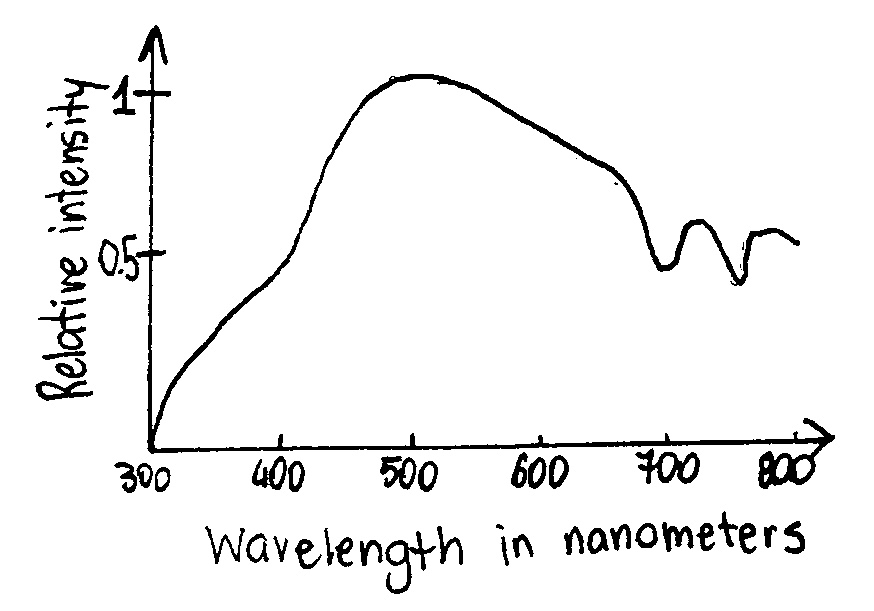
\includegraphics[height=4cm]{pbr/spectrum.jpg}
  \caption{Widmo światła widzialnego emitowanego przez Słońce}
\end{figure}

Oddziaływanie światła z materią jest opisane przez wielkość nazywaną współczynnikiem załamania $n$. Współczynnik załamania mówi nam, jak materia wpływa na prędkość światła oraz w postaci rozszerzonej w której współczynnik jest wartością zespoloną również pozwala obliczyć jak dużo światła jest absorbowanego w danym ośrodku. Podstawowym wzorem na $n$ jest:
\[
    n = \frac{c}{v}
\]
gdzie $c$ jest prędkością światła w próżni ($\SI{2.998e8}{\meter\per\second}$), a $v$ prędkością fazową fali, czyli prędkością z jaką faza propaguje się w przestrzeni.

Najprostszym rodzajem ośrodka jest medium jednorodne, które ma jednolitą strukturę wewnętrzną o stałym współczynniku załamania. Na skutek tego prędkość światła w każdym punkcie i dowolnym kierunku jest jednakowa. W takim przypadku światło w ośrodku porusza się w linii prostej. Najlepszym przykładem ośrodka tego typu jest próżnia. Mimo braku zmiany kierunku w większości ośrodków następuje utrata energii na skutek absorpcji wynikającej ze zderzeń z atomami materii. Nawet niewielki stopień utraty energii może skutkować całkowitym jej pochłonięciem na większym dystansie np. pod wodą. Innym przykładem medium jednorodnego o niskiej absorpcji jest szkło i powietrze.

Ośrodkiem niejednorodnym nazywamy ośrodek o niejednorodnej strukturze wewnętrznej w którym prędkość światła jest zależna od kierunku lub badanego miejsca - w związku z czym współczynnik załamania jest zależny od pozycji w ośrodku. Jeżeli w otoczeniu danego punktu współczynnik załamania zmienia się to promień przechodzący przez ten punkt zmieni swój kierunek. W przypadku ciągłej zmiany współczynnika promień zostanie zagięty, jednak dla nieciągłości nastąpi podział wiązki na dwie części - na część refrakcyjną oraz odbitą. Część odbita nie opuści obecnego ośrodka, lecz zmieni kierunek i wróci do jego wnętrza. Część refrakcyjna natomiast zostanie zagięta oraz przejdzie do drugiego ośrodka. 

W bardzo różnorodnych strukturach może dojść do sytuacji w której na skutek dużej ilości nieciągłości lub znacznych wahań współczynnika załamania światło  zostanie wymieszane tak, że promienie będą podążały w losowych kierunkach. Takie zjawisko będziemy nazywać rozpraszaniem (ang. \textit{scattering}). Przykładem substancji w której łatwo je zaobserwować jest mleko.

Warto w tym miejscu zastanowić się nad znaczeniem skali dla rozpraszania światła. Małe zaburzenia w niewielkim otoczeniu mogą nie mieć dużego wpływu na fale świetlne, lecz w dużej skali nie mogą zostać pominięte. Czyste powietrze nie powoduje mieszania się światła na krótkich dystansach, jednak nawet taki ośrodek powoduje znaczne rozproszenie, gdy bierzemy pod uwagę sceny w których można dostrzec punkty leżące wiele kilometrów od obserwatora. 

Oprócz jednorodności lub niejednorodności możemy podzielić substancje na trzy główne kategorie, są to:

\begin{itemize}
	\item przewodniki (metale) - materiały dobrze przewodzące prąd elektryczny, przykładami przewodników są: grafit, żelazo, stal, aluminium, złoto, miedz
    
	\item izolatory (dielektryki) - materiały w których prąd elektryczny przewodzony jest bardzo słabo, jest to rezultatem niskiej koncentracji ładunków swobodnych i/lub zbyt małej ich ruchliwości, przykładami dielektryków są szkło, ceramika, tworzywa sztuczne, suche drewno, powietrze
	
	\item półprzewodniki - substancje, dla których przewodnictwo prądowe może być zmieniane w szerokim zakresie. Ze względu na ich rzadkie występowanie w codziennym otoczeniu (poza środowiskami laboratoryjnymi), nie będziemy ich brać pod uwagę. W przypadku konieczności wymodelowania materiału półprzewodnikowego możemy zbudować wystarczający w wielu przypadkach model będący interpolacją między przewodnikiem a izolatorem
\end{itemize}

Metale oraz dielektryki posiadają kilka szczególnych właściwości, które muszą zostać wzięte pod uwagę podczas obliczeń. Różnice zostaną przedstawione nieco później w tym rozdziale.

Zrozumienie sposobu w jaki wiązka światła zachowuje się po zderzeniu z idealnie równą powierzchnią jest fundamentem całej dziedziny metod opartych na prawach fizycznych. Dopóki nie wprowadzimy pojęcia chropowatości będziemy zakładać, że analizowana powierzchnia jest optycznie gładka tzn. że wszystkie nierówności na tej powierzchni są mniejsze niż długość aktualnie analizowanej fali (mniejsze niż $400-700$nm) przez co możemy przyjąć, że nie wpływają one w żaden sposób na zachowanie promieni.

Dla uproszczenia objaśnień będziemy również zakładać, że analizowany materiał nie emituje światła. Dodanie emisji energii nie powinno stanowić żadnego problemu po zbudowaniu modelu dla interakcji z zewnętrznymi źródłami światła.

Wiązka światła podczas zderzenia z powierzchnią (dokładniej, przy przejściu z jednego ośrodka do drugiego, w miejscu w którym występuje nieciągłość współczynnika załamania) rozdziela się na dwie części: część odbitą od powierzchni oraz załamaną (część która ulega refrakcji).

Reflektancją powierzchniową $\mathbb{R}_{\text{surf}}$ \cite{pbr_games_siggraph} będziemy nazywać stosunek natężenia światła odbitego $I_o$ do światła przychodzącego $I_i$ w danym punkcie dla danej długości fali $\lambda$:
\[
	\mathbb{R}^{\text{surf}}(\lambda) = \frac{
        I_o
    }{
        I_i
    } \in \left[
        0, 1 
    \right]
\]

Reflektancja powierzchniowa zależna jest również od kąta padania promienia oraz długości fali. Reflektancję dla kąta padania równego $\ang{0}$ będziemy oznaczać poprzez $\mathbb{R}^{\text{surf}}_{0}$ - ta wartość bardzo często używana jest jako wartość bazowa dla modeli przybliżających wartość reflektancji dla wszystkich kątów. 

Różnice między metalami a izolatorami rozpoczynają być widoczne przy analizie reflektancji powierzchniowej. Wartość $\mathbb{R}^{\text{surf}}_{0}$ dla izolatorów zwykle nie przekracza 6\%. Sytuacja wygląda zupełnie inaczej w świecie metali, wartość reflektancji powierzchniowej dla kierunku zgodnego z normalną tej powierzchni ($\mathbb{R}^{\text{surf}}_{0}$) jest zazwyczaj wyższa niż 50\%.

Część energii, która została uległa refrakcji wchodzi wgłąb, gdzie zachodzą kolejne kolizje z atomami materii, przez co znów dochodzi do wyżej wspomnianego zjawiska podziału promienia, tym razem we wnętrzu badanego ciała. Część tego światła może wydostać się ponownie z obiektu do ośrodka źródłowego, pozostała część zostanie pochłonięta i zamieniona na inne rodzaje energii np. ciepło.

Ilość światła, które wydostaje się z powrotem z wnętrza ciała jest zależna od rodzaju substancji z której jest wykonany obiekt. Dla metali część światła, która dostaje się do wnętrza zostaje bardzo szybko pochłonięta przez wolne elektrony i zamieniona na ciepło. Z tego względu światło które ulega refrakcji nie wydostanie się z tego metalu. Wnioskiem jest to, że na wygląd metali wpływają jedynie promienie które zostają odbite od jego powierzchni. Dla dielektryków sytuacja wygląda inaczej, ze względu na budowę atomową światło nie jest pochłaniane w dużym stopniu i bardzo często jest uwolnione w innym miejscu ciała.

W modelach matematycznych wymienionych w tej pracy zakładamy, że ponowne wyjście energii która była poddana refrakcji następuje lokalnie tzn. w powierzchni, która przypada na obecnie generowany piksel dla którego promień zderzył się z powierzchnią (rys. \ref{fig:ReflectionRefraction}).

% Rysunek odbicia z płaską powierzchnią (model uproszczony)
\begin{figure}[h]
  \centering
  \begin{tikzpicture}
    %\draw[help lines] (-5,-1) grid (5,5);
    \draw [thick] (-5.0,0.0) -- (5.0,0.0);

    % Specular
    \foreach \i in {0,...,5} {
      \pgfmathtruncatemacro{\angle}{90+30+(\i / 5) * 30};
      \draw [-Triangle, blue] (0,0) -- ( {3*cos(\angle)}, {3*sin(\angle)} );
    }

    % Diffuse
    \foreach \i in {1,...,15} {
      \pgfmathtruncatemacro{\angle}{(\i / 16) * 180};
      \draw [-Triangle, gray] (0,0) -- ( {2*cos(\angle)}, {2*sin(\angle)} );
    }

    \draw [fill] (2,2) circle [radius=0.05] node [above] {\Large\faLightbulbO};
    \draw [-{Triangle[scale=2]}] (2,2) -- (0,0);
  \end{tikzpicture}
  \caption{Przybliżony model interakcji wiązki światła z powierzchnią}
  \label{fig:ReflectionRefraction}
\end{figure}

Istnieją techniki które biorą pod uwagę możliwość ucieczki energii w dalej położonym miejscu miejscu, ale skomplikowałyby one rozważania na których skupia się ta praca. Takie techniki muszą operować globalnie i zakładać możliwość wpływu obszaru przypadającego na jeden piksel na drugi. Wymagane są one do uzyskania realistycznych obrazów w którym pojawiają się materiały takie jak skóra, wosk i inne w których rozproszenie podpowierzchniowe jest wyraźnie widoczne. Zauważmy znowu, że rozważanie tego, czy dany materiał wymaga globalnej metody na wyznaczenie ucieczki światła z wnętrza materii jest zależne od skali. Jeżeli będziemy obserwować plastik, który w wymiarze standardowym dla gier nie wykazuje żadnych widocznych ,,interakcji'' między pikselami, to nie oznacza, że będzie tak również dla bardzo dużego przybliżenia tej powierzchni. Podobnie rozpalona woskowa świeczka lub marmurowa rzezba zmniejszona do bardzo małych rozmiarów nie będzie wykazywała istnienia takiego zjawiska.

Reflektancja powierzchniowa nie bierze pod uwagę światła uciekającego z wnętrza ciała. Dlatego też, zdefiniujemy dodatkowe pojęcie które będziemy nazywać reflektancją ciała lub objętości (ang. \textit{body/volume reflectance}). Definicja będzie analogiczna do poprzedniej: reflektancją objętośći $\mathbb{R}^{\textit{vol}}$ będziemy nazywać stosunek ilości światła wychodzącego do przychodzącego w bardzo małym obszarze w danym punkcie. W przeciwieństwie do reflektancji powierzchniowej wartość reflektancji objętościowej jest bardzo zróżnicowana, wartość ta dla śniegu wynosi około 80\%, dla kamienia około 20\%, a dla węgla blisko 0\%.

Zauważmy, że w przypadku braku emisji energii oraz przy lokalnej ucieczce światła z materii energia która dociera doobserwatora musi być mniejsza lub równa energii wiązki światła - ta właściwość jest jednym z filarów modeli opartych na zjawiskach fizycznych.

\begin{figure}[ht]
  \centering
  \begin{tikzpicture}
    %\draw[help lines] (-5,-1) grid (5,5);

		\coordinate (left) at (-3,0);
		\coordinate (right) at (3,0);
    \draw [ultra thick] (left) -- (right);

		\coordinate (normal) at (0,3);
		\coordinate (invnormal) at (0,-3);

    \draw  [-{Triangle[scale=2]}] (invnormal) -- (normal) node [above] {$N$};

		\coordinate (orig) at (0,0);
		\coordinate (light) at (45:3);
		\coordinate (reflection) at (135:3);
		\coordinate (refraction) at (205:3);

    \draw  [-{Triangle[scale=2]}] (orig) -- (reflection)
      node [midway, above] {$r$};
    \draw  [-{Triangle[scale=2]}] (orig) -- (refraction)
      node [midway, above] {$t$};
    \draw  [-{Triangle[scale=2]}] (light) -- (orig);

    \draw pic[draw=black, <->, "$\alpha_i$", angle eccentricity=1.5]
			{angle = light--orig--normal};

    \draw pic[draw=black, <->, "$\alpha_r$", angle eccentricity=1.5]
			{angle = normal--orig--reflection};

    \draw pic[draw=black, <->, "$\beta$", angle eccentricity=1.5]
			{angle = refraction--orig--invnormal};

    \node at (2.8,+0.25) {$n_1$};
    \node at (2.8,-0.25) {$n_2$};

    \draw [fill] (light) circle [radius=0.05] node [above] {\Large\faLightbulbO};

  \end{tikzpicture}
  \caption{Przybliżony model interakcji wiązki światła z powierzchnią}
  \label{fig:ReflectionRefractionDetailed}
\end{figure}

Do określenia tego ile i w jaki sposób wiązka światła będzie oddziaływać z powierzchnią poprzez odbicie lub refrakcję będziemy potrzebować kilku podstawowych praw fizycznych. Notacja wykorzystana we wzorach jest zgodna ze schematem z rys. \ref{fig:ReflectionRefractionDetailed}.

Podstawowym prawem wykorzystywanym do analizy zachowania wiązki światła jest prawo wiążące kąt padania oraz kąt odbicia promienia. Kąty padania wiązki światła $\alpha_i$ i jej odbicia $\alpha_r$ od płaszczyzny (zatem od idealnie gładkiej powierzchni) są równe ($\alpha_i = \alpha_r = \alpha$).


Zmiana kierunku promienia światła przy przejściu przez granicę dwóch ośrodków jednorodnych o współczynnikach załamania $n_1, n_2$ opisana jest równaniem Snella:
\[
\frac{\sin\alpha}{\sin\beta} =
  \frac{n_2}{n_1} = n_{21}
\]

Stosunek energii wiązki światła odbitego do załamanego opisany jest równaniami Fresnela będących rozwiązaniem równań Maxwella dla fal świetlnych przechodzących przez jednorodne ośrodki o różnych współczynnikach załamania przez idealnie płaską granicę. W tej pracy nie będziemy korzystać bezpośrednio z równań Fresnela, lecz z ich aproksymacji, w szczególności z aproksymacji Schlicka. Współczynnik Fresnela, jego znaczenie i opis aproksymacji zostanie przedstawione dalej w tym rozdziale.

Te trzy prawa pozwalają nam na opis zachowania światła wystarczający do zastosowań w grafice czasu rzeczywistego.

W naturze mało, który materiał jest optycznie idealnym lustrem (tak abyśmy mogli zastosować tutaj uproszczone równania Fresnela), w odpowiednio dużym przybliżeniu realnych pozornie gładkich powierzchni zauważymy nierówności niedostrzegalne gołym okiem, a jednocześnie wpływające znaczące na ogólny wygląd powierzchni (rys. \ref{fig:Microstructure}). Im większa jest nierówność tym większe jest zróżnicowanie normalnych w tym otoczeniu. W związku z tym światło się bardziej miesza i refleksy są coraz mniej wyraźne. Nierówności powierzchni wpływające na jej wygląd lecz nieobserwowalne w badanej skali będziemy nazywać mikrogeometrią lub mikrostrukturą.

\begin{figure}[ht]
  \centering
  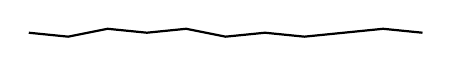
\begin{tikzpicture}
    \draw [thick]
      (0.0,0.15) --
      (0.5,0.10) --
      (1.0,0.20) --
      (1.5,0.15) --
      (2.0,0.20) --
      (2.5,0.10) --
      (3.0,0.15) --
      (3.5,0.10) --
      (4.0,0.15) --
      (4.5,0.20) --
      (5.0,0.15);
  \end{tikzpicture}
  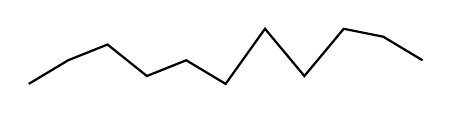
\begin{tikzpicture}
    \draw [thick]
      (0.0,0.1) --
      (0.5,0.4) --
      (1.0,0.6) --
      (1.5,0.2) --
      (2.0,0.4) --
      (2.5,0.1) --
      (3.0,0.8) --
      (3.5,0.2) --
      (4.0,0.8) --
      (4.5,0.7) --
      (5.0,0.4);
  \end{tikzpicture}
  \vspace{0.25cm}
  \caption{Mikrostruktury powierzchni o różnej chropowatości}
	\label{fig:Microstructure}
\end{figure}

Warto zauważyć, że nawet jeżeli wiązka światła odbija się w kierunku obserwatora nie oznacza to, że wyjdzie z otoczenia powierzchni i do niego trafi. Mała nierówność może spowodować zasłonięcie obserwatora z perspektywy tego punktu i odbić się ponownie w zupełnie innym kierunku. Będziemy wtedy mówić o maskowaniu (ang. \textit{masking}). Modele bazujące na mikro-powierzchniach zazwyczaj nie biorą pod uwagę odbić wielokrotnych i to takimi modelami odbić jednokrotnych (ang. \textit{single-bounce models}) będziemy się zajmować. Wielokrotne odbicie w mikrostrukturze (ang. \textit{multiple-bounce model}) jest wciąż problemem otwartym, nie istnieją jeszcze zrozumiałe i powszechnie akceptowane modele opisujące to zjawisko.

Możliwa jest również sytuacja odwrotna, w której dany punkt może być teoretycznie zaobserwowany przez obserwatora, ale światło nie dociera do tego punktu na skutek przysłaniania źródła światła przez sam obiekt (samo-zacienianie, ang. \textit{shadowing}).

\missingfigure{Rysunek samozaciemniania moze tutaj?}

\section{Podstawowe pojęcia radiometryczne}

Rozpocznijmy od podstawowego budulca wiązki światła - fotonu. Energia pojedynczego fotonu o długości fali $\lambda$ może zostać obliczona przy użyciu wzoru:
\[ 
    Q = \frac{hc}{\lambda} 
\]
\noindent gdzie $h$ jest stałą Plancka ($\SI{6.62620e-34}{\joule\per\second}$), a $c$ prędkością światła w próżni. Wszystkie kolejne miary przedstawione w tej sekcji są funkcją długości fali.

Strumień promieniowania (inaczej moc promieniowania, ang. \textit{radiant flux}) to całkowita ilość energii przechodząca przez określoną powierzchnię w czasie jednostkowym. Powyższe pojęcie dotyczy wszystkich fal elektromagmetycznych, zatem jest ono poprawne również dla światła. Jednostką strumienia promieniowania jest Watt ($\si{\watt}$).
\[
\Phi = 
    \lim_{\Delta t \rightarrow 0}{
        \frac{\Delta Q}{\Delta t}
    } 
    = \frac{\dd Q}{\dd t}
\]

Radiancją wyjściową (ang. \textit{radiant exitance, radiosity}) $B$ nazywamy wyemitowany strumień promieniowania $\Phi_{e}$ przez powierzchnię na jej powierzchnię jednostkową:
\[
B(p) = 
    \lim_{\Delta \rightarrow 0}{
        \frac{\Delta \Phi_{e}(p)}{\Delta A}
    } 
    = \frac{\dd \Phi_{e}}{\dd A}
\]  

Irradiancją (ang. \textit{irradiance}) nazywamy strumień promieniowania przychodzącego $\Phi$ na jednostkę powierzchni:
\[
E(p) =
    \lim_{\Delta \rightarrow 0} {
        \frac{\Delta \Phi(p)}{\Delta A}
    } =
    \frac{\dd \Phi(p)}{\dd A}
\]

Oczywiście całkując irradiancję na powierzchni otrzymamy z powrotem strumień promieniowania:
\[
\Phi = \int_{A} {
    E(p)
    \dd A
}
\]

W tym miejscu warto zauważyć, że jeżeli powierzchnia $A$ jest nachylona do
strumienia światła $\Phi$ pod pewnym kątem $\alpha$ to irradiancja zmienia się
proporcjonalnie do czynnika $\cos \alpha$. Wynika to z faktu, że obszar na
który padają promienie emitowane przez źródło światła w kierunku prostopadłym
do powierzchni tego źródła jest zależny od kąta pod którym nachylona jest
powierzchnia (rys. \ref{fig:SourceLightAngle}). Powierzchnia ta jest odwrotnie
proporcjonalna do czynnika $\cos \alpha$, zatem dzieląc przez powierzchnię
otrzymujemy zależność wprost proporcjonalną dla irradiancji.

\begin{figure}[ht]
  \centering
  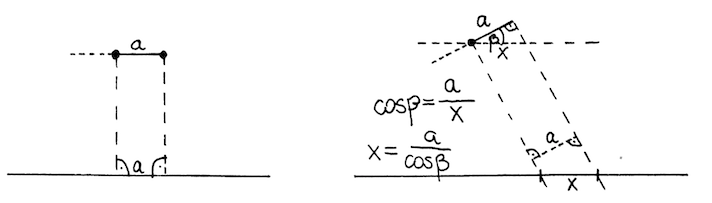
\includegraphics[height=3cm]{pbr/sourcelightangle.png}
  \caption{Wpływ kąta na powierzchnię na które oddziaływuje światło}
  \label{fig:SourceLightAngle}
\end{figure}

W przypadku jednorodnym irradiancję możemy zdefiniować jako średnią moc
promieniowania na pewnej skończonej powierzchni $A$:
\[
    E = \frac{\Phi}{A}
\]

\begin{example}
  Irradiancja dla światła punktowego w punkcie $p$ na sferze o
  promieniu $r$ o środku w tym właśnie punkcie $p$ wynosi:
  \[
    E = \frac{\Phi}{4 \pi r^2}
  \]
\end{example}

Kątem planarnym obiektu geometrycznego $G$ z punktu $p$ nazywamy ,,kąt'' wyznaczony przez dwie półproste rozpoczynające się w punkcie $p$ wyznaczające minimalny obszar zawierający obiekt $G$. Miarą kąta planarnego jest \textit{radian} (\si{\radian}). Inaczej mówiąc, kąt jest ciągłym zbiorem kierunków na płaszczyznie, a jego rozmiar jest równy długości łuku wyznaczonego przez wektory jednostkowe odpowiadające tym kierunkom.

% Rysunek kąta geometrycznego
\begin{figure}[ht]
  \centering
  \begin{tikzpicture}
    \coordinate (orig) at (0,0);
    \coordinate (left) at (1,3);
    \coordinate (right) at (5,2);
    \draw (2,1) -- (left) -- (2,4) -- (right) -- (2,1);
    \draw [dashed] (left)--(orig)--(right);
    \draw [fill] (orig) circle [radius=0.08] node [below] {$p$};
    \draw pic[draw=black, <->, "$\theta$", angle eccentricity=1.5] {angle = right--orig--left};
  \end{tikzpicture}
  \caption{Kąt planarny obiektu geometrycznego}
  \label{fig:PlanarAngle}
\end{figure}

Kąt bryłowy jest rozszerzeniem kąta planarnego do trzech wymiarów. Kątem bryłowym $A$ nazywamy ciągły zbiór kierunków w przestrzeni trójwymiarowej mierzony polem powierzchni obszaru zdefiniowanego przez wektory jednostkowe odpowiadające tym kierunkom. Kątem bryłowym możemy też nazwać powierzchnię rzutu trójwymiarowego obiektu geometrycznego $G$ na sferę jednostkową o środku w punkcie $p$. Jest on mierzony w steradianach (\si{\steradian}). Kąt bryłowy całej sfery jednostkowej wynosi $\SI{4\pi}{\steradian}$.

% Rysunek kąta bryłowego
\begin{figure}[ht]
  \centering
  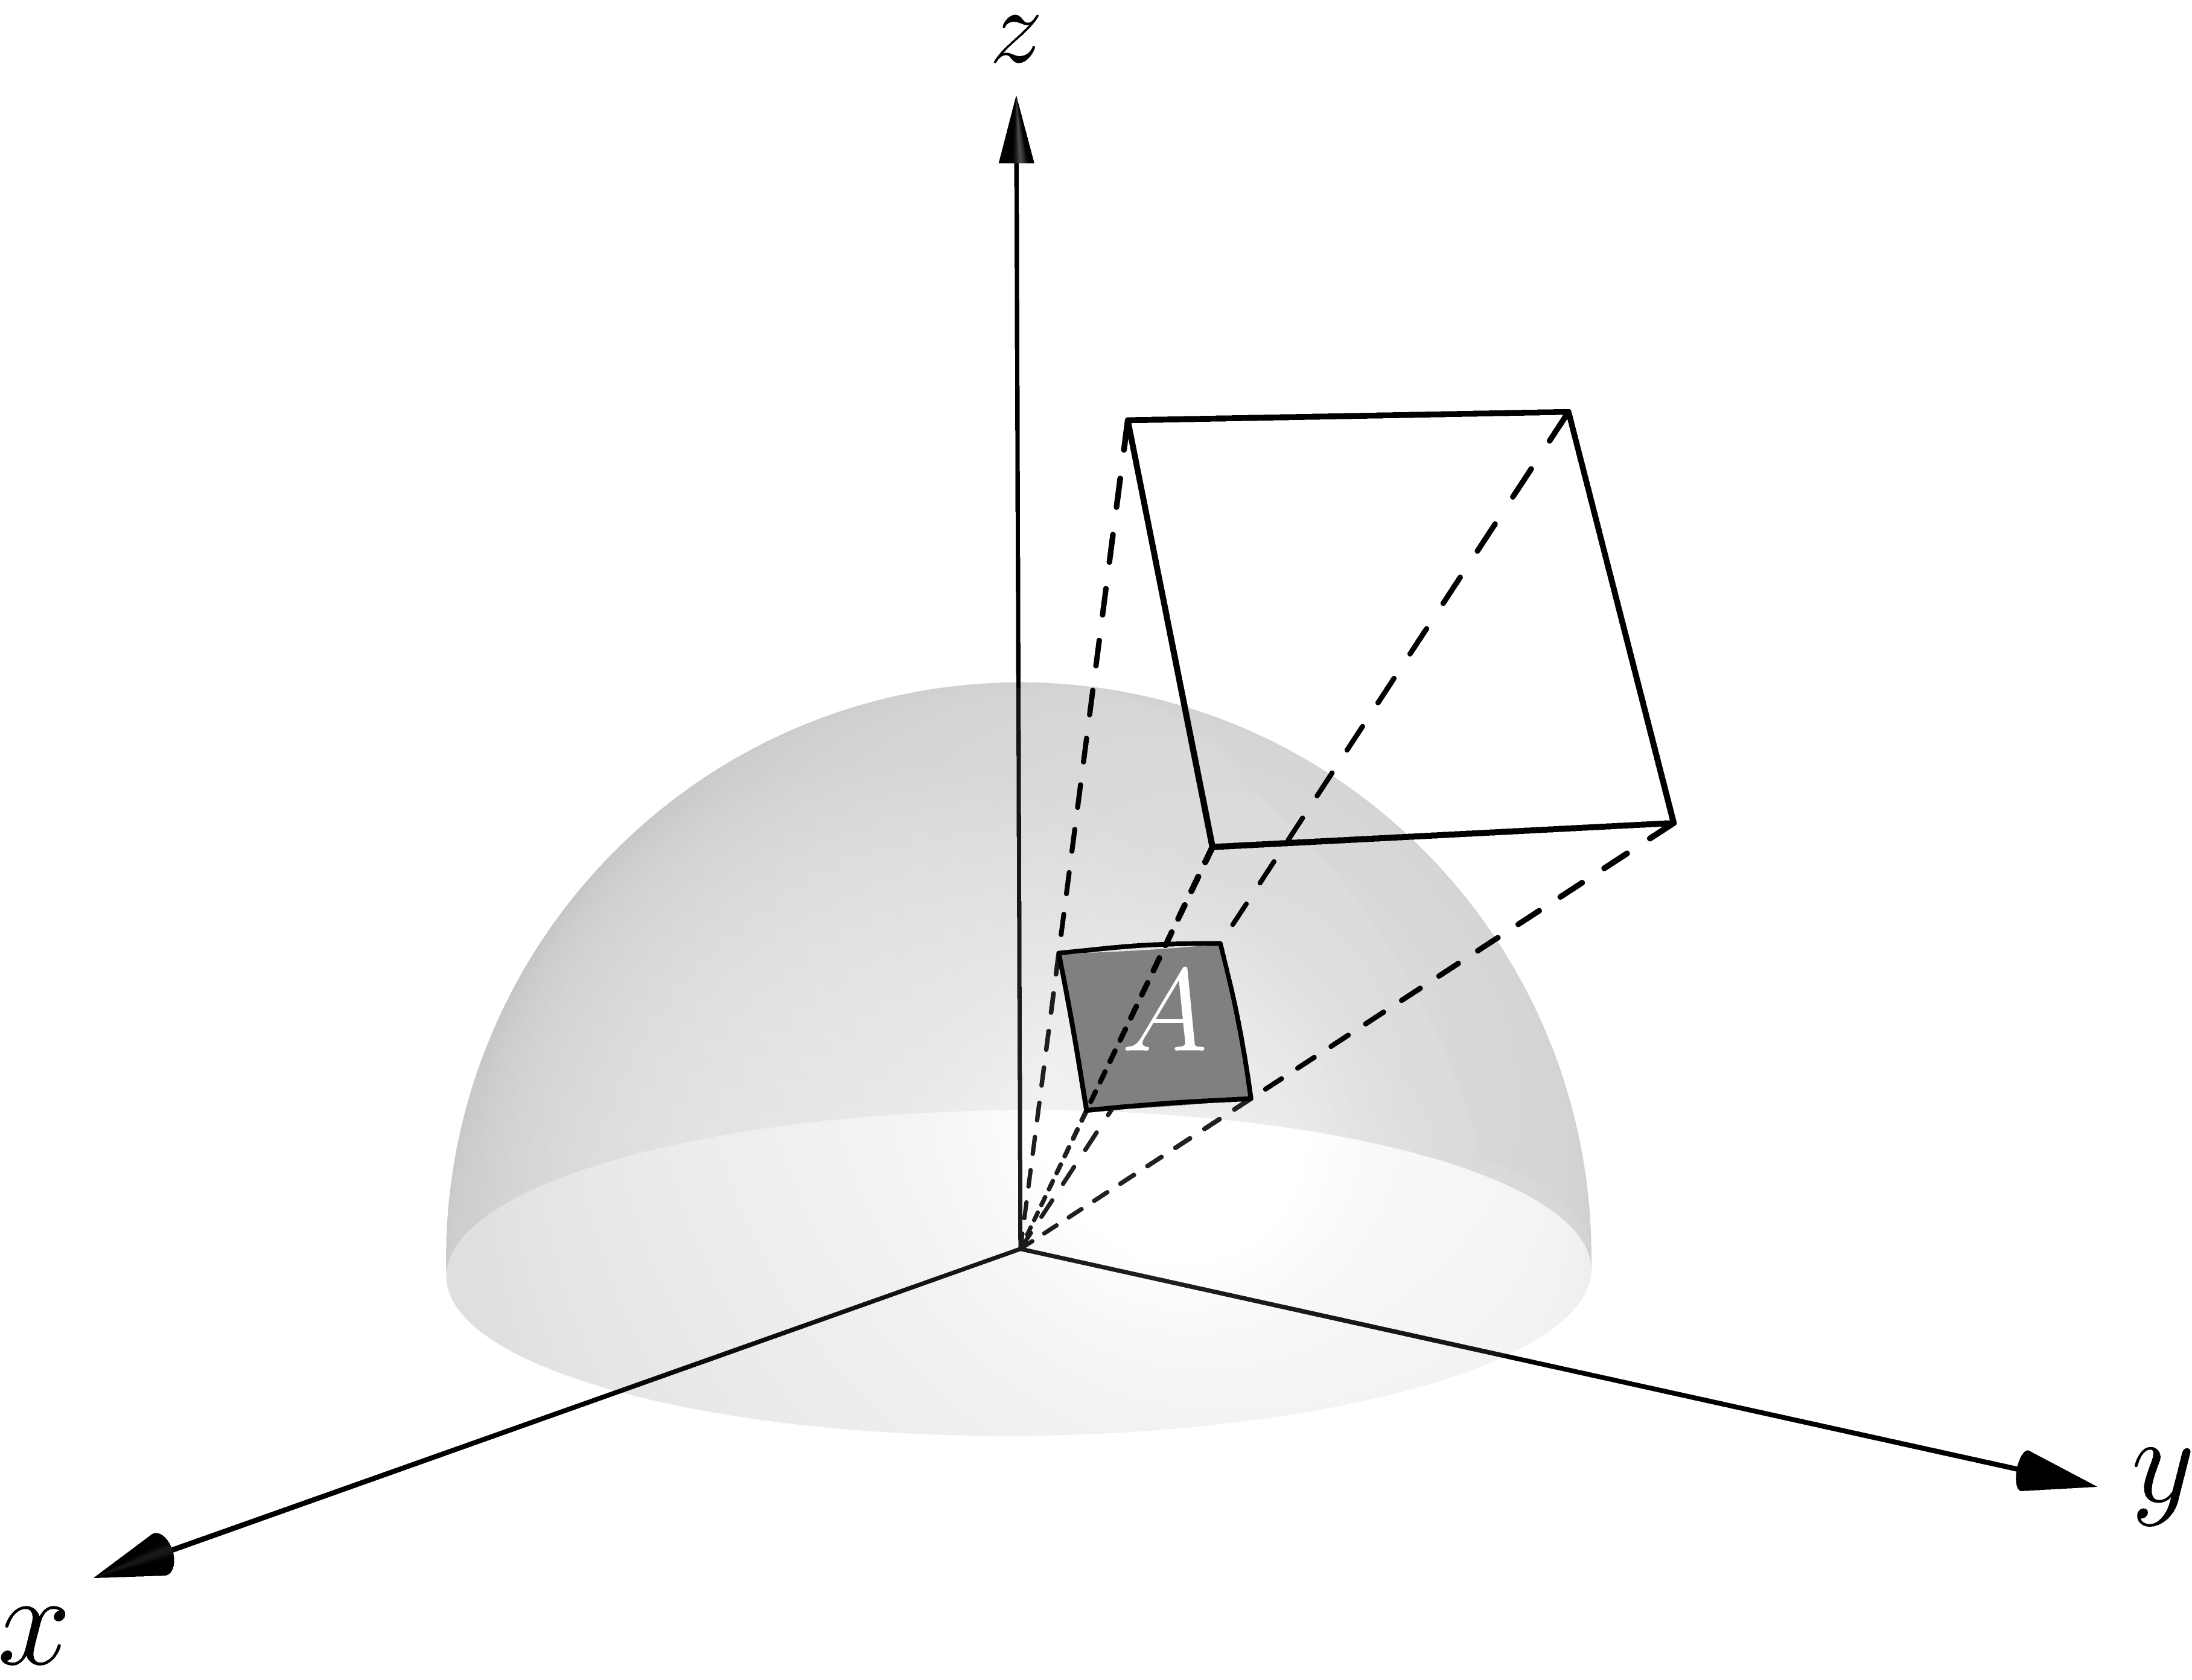
\includegraphics[height=5cm]{pbr/solid_angle.png}
  \caption{Kąt bryłowy powierzchni}
  \label{fig:SolidAngle}
\end{figure}

Kolejną miarą energii jest intensywność źródła (ang. \textit{intensity}), która reprezentuje rozkład gęstości mocy światła na kierunkach \cite[p. 328]{pbrt}. Warto na wstępie zauważyć, że intensywność ma sens tylko i wyłącznie dla teoretycznych świateł punktowych lub bardzo odległych które możemy traktować jako kierunkowe ze względu na sposób pomiaru kąta. Wartość tą możemy zdefiniować w następujący sposób:
\begin{gather*}
  I = \lim_{\Delta\omega \rightarrow 0} {
    \frac{\Delta\Phi}{\Delta\omega}
  } = \frac{d\Phi}{d\omega} \\
  \Phi = \int_{\Omega} {I(\omega) d\omega}
\end{gather*}
\noindent gdzie przez $\omega$ rozumiemy wektor określający kierunek ze środka
jednostkowej sfery do punktu leżącego na jej brzegu.

Dla przykładu intensywność teoretycznego jednorodnego światła punktowego wynosi:
\[
  I = \frac{\Phi}{4\pi}
\]

Poprzez $E_{\omega}$ oznaczmy irradiancję hipotetycznej powierzchni
prostopadłej do kierunku $\omega$. Radiancją (ang. \textit{radiance}) $L$ nazywamy miarę irradiancji $E_{\omega}$ w odniesieniu do kąta bryłowego:
\[
L(p, \omega) = \lim_{\Delta\omega \rightarrow 0} {
  \frac{\Delta E_{\omega} (p)}{\Delta\omega}
} =
\frac{\dd E_{\omega}(p)}{\dd \omega}
\]

Bardzo ważną obserwacją jest to, że radiancja nie jest mierzona względem irradiancji powierzchni na której leży punkt $p$, ma to na celu wyeliminowanie czynnika $\cos \alpha$ z definicji \cite[p. 339]{pbrt}. Jednostką radiancji jest gęstość energii na jednostkę powierzchni na jednostkę kąta bryłowego. Radiancję możemy interpretować jako miarę ilości światła wzdłuż jednego
promienia.

Irradiancję (tutaj względem normalnej makro-powierzchni) możemy odzyskać całkując radiancję ponownie względem makro-powierzchni (stąd czynnik $\cos\theta$):
\begin{gather*}
    \dd E = L(p, \omega) \cos\theta \dd \omega \\
    E = \int_{\Omega_H}{L(p, \omega) \cos\theta \dd \omega}
\end{gather*}

Funkcja \textit{BRDF} (ang. \textit{Bidirectional Reflectance Distribution Function}) wyznacza stosunek irradiancji do odbitej radiancji:
\[
f_r(\omega_i, \omega_o) = \frac{
    \dd L_{o}(\omega_o)
}{
    \dd E(\omega_i)
}
\]
\noindent Jednostką BRDF jest $\si[per-mode=reciprocal]{\per\steradian}$.

\section{Równanie renderingu}

\textbf{Równanie renderingu} (ang. \textit{rendering equation}) to równanie
całkowe określające radiancję wychodzącą z danego punktu $p$ w danym kierunku
$\omega_o$ znając radiancję przychodzącą do tego punktu. Równanie te możemy
wyprowadzić z poprzednio przedstawionych definicji:
\begin{gather*}
    f_r(\omega_i, \omega_o) = \frac{
        \dd L_{o}(\omega_o)
    }{
        \dd E(\omega_i)
    } \Rightarrow 
    \dd L_{o}(\omega_o) =  f_r(\omega_i, \omega_o) \dd E(\omega_i) \\
    \dd E(\omega_i) = L_i(p, \omega) \cos\theta \dd\omega
\end{gather*}

Podstawiając drugie równanie do pierwszego i całkując otrzymujemy:
\[
  L_{o}(\omega_o) =
  \int_{\Omega} {
    f_r(p, \omega_i, \omega_o)
    L_i(\omega_i)
    (n \cdot \omega_i)
    \dd{\omega_i}
  }
\]

\noindent gdzie poszczególne składowe to:

\begin{itemize}

  \item $L_i(\omega_i)$ - radiancja przychodząca z kierunku $\omega_i$

  \item $\Omega$ - jednostkowa półsfera wyznaczająca dziedzinę wszystkich
    możliwych kierunków przychodzących $\omega_i$

  \item $f_{r}(p, \omega_i, \omega_o)$ - funkcja \textit{BRDF} (ang.
    \textit{Bidirectional Reflectance Distribution Function}) wyznaczająca jaka
    część energii przybywającej z kierunku $\omega_i$ zostanie wysłana w zadanym kierunku $\omega_o$

\end{itemize}

Bardzo często wykorzystywaną formą tego równania jest postać z parametryzacją polarną kątami $\phi$ i $\theta$. W takim przypadku $\dd \omega$ jest równe $\sin\theta \dd\theta \dd\phi$ \cite{wolfram_solidangle} stąd uzyskujemy:
\[
L_{o}(\theta_o, \phi_o) = \int_{0}^{2\pi} \int_{0}^{\frac{\pi}{2}} {
	f(\theta_i, \phi_i, \theta_o, \phi_o)L(\theta_i, \phi_i) \cos\theta_i \sin\theta_i
} \dd\theta_i \dd\phi_i
\]

\noindent Postać jest szczególnie istotna w zastosowaniach praktycznych.

\section{Bidirectional Reflectance Distribution Function}

Aby funkcja BRDF była fizycznie wiarygodna (ang. \textit{physically plausible})
musi spełniać dwa warunki. Po pierwsze, funkcja BRDF musi być niezależna od
kolejności parametrów, odwrócenie wszystkich kierunków promieni powinno dać nam
dokładnie ten sam wynik (ang. \textit{Helmholtz reciprocity}):

\[
  \forall{\omega_i, \omega_o \in \Omega} \quad
  f_r(\omega_i, \omega_o) = f_r(\omega_o, \omega_i)
\]

Po drugie, funkcja BRDF nie może emitować więcej światła niż otrzymuje (pamiętajmy o załozeniu braku emisji). Kierunkowa reflektancja półsferyczna (ang. \textit{directional-hemispherical reflectance}) $R(\omega_i)$ jest kolejną funkcją związaną z BRDF mierzącą ile energii przychodzącej z danego kierunku $\omega_i$ zostanie odbite w jakimkolwiek innym kierunku. Inaczej mówiąc, mierzy ona straty lub zyski energii dla danego kierunku wejściowego. Zauważmy, że dla modeli spełniających warunek zachowania energii wartość ta musi być w przedziale $\left[0,1\right]$ dla każdej długości fali $\lambda$ i kierunku przychodzącego $\omega_o$. Funkcja ta zdefiniowana jest w sposób następujący \cite{RealTimeRendering2008}:
\[
  R(\omega_i) 
  = \frac{\dd B}{\dd E(\omega_i)} 
  = \int_{\Omega} {
    f_r(\omega_i, \omega_o)
    (n \cdot \omega_o)
    \dd \omega_o
  }
\]

W tym miejscu warto wprowadzić kolejną wielkość nazywaną albedo lub bi-półsferyczną reflektancją (ang. \textit{bihemispherical reflectance, albedo}) zdefiniowaną jako stosunek całkowitego \textit{radiant exitance} do irradiancji.
\[
    \rho = \frac{B}{E} = \frac{1}{\pi} \int_{\Omega}{
        R(\omega_i) \cos\theta_i d\omega_i
    }
    = \frac{1}{\pi} \int_{\Omega} \int_{\Omega} {
        f_r(\omega_i, \omega_o) 
        \cos\theta_i 
        \cos\theta_o 
        \dd\omega_i 
        \dd\omega_o
    }
    \in \left[0, 1\right]
\]

Albedo jest bardzo użyteczną miarą, którą można interpretować jako ogólny stopień refleksywności danej powierzchni. Parametr ten bardzo często jest wykorzystywany jako parametr wejściowy systemu oświetlenia.

Cała funkcja BRDF zwykle zawiera część opisującą reflektancję powierzchniową (specular) oraz część dla reflektancji ciała (rozproszoną), przez co większość modeli rozdziela je i analizuje osobno lub definiuje tylko jeden fragment możliwy do wykorzystania z innym. Do podziału wiązki światła przy zderzeniu najczęściej używane są równania Fresnela.

Istnieje bardzo dużo róznych modeli BRDF \cite{brdf_overview}, my zajmiemy się natomiast kilkoma wybranymi.

\subsection{Lambert}

Najprostszą funkcją BRDF jest rozkład jednorodny, niezależny od kąta obserwacji. Taka funkcja jest rozkładem lambertowskim opisanym poniższym równaniem:
\[
  f_r = \frac{\rho}{\pi}
\]
\noindent gdzie $\rho$ to albedo, które możemy interpretować jako kolor rozproszony. Wyprowadzenie tego można znaleźć w \cite{RealTimeRendering2008}\cite{pbr_games_siggraph}, wynika ono z założenia, że BRDF dla każdego kierunku jest równy.

Model ten bardzo często jest wykorzystywany do opisania części rozproszonej wielu modeli BRDF, szczególnie do modelowania gładkich dielektryków. Wartość $\rho$ (albedo) jest również często oznaczana poprzez $\text{c}_{\text{diff}}$ i jest ona rozumiana jako kolor rozproszony powierzchni (ang. \textit{diffuse color}).

Teoretyczna powierzchnia lambertowska odbija tą samą ilość radiancji w każdym kierunku. Warto w tym miejscu zauważyć, czynnik równy kosinusowi kąta padania światła kojarzony z modelem Lamberta jest częścią równania renderingu, a nie samej funkcji BRDF.

Bardzo często w rzeczywistych aplikacjach czynnik $\pi^{-1}$ nie występuje, ze względu na to, że zostaje on wliczony do ,,irradiancji'' światła, przez co efektywnie jest ona mniejsza niż powinna być wg. rachunków radiometrycznych. 

\subsection{Minnaert}

Alternatywnym modelem dla gładkich izotropowych powierzchni jest model
Minnaert'a. Model ten został stworzony do opisu powierzchni księżyca, można
spotkać się z określeniem modelu księżycowego (ang. \textit{moon shading}).
Główną zmianą jest zależność jasności od kąta obserwacji i kąta padania światła
na powierzchnię.  Model ten jest szczególnie przydatny do obliczenia
oświetlenia dla aksamitu, dywanów. Model ten opisany jest wzorem:
\[
  f_r = \frac{\rho_d}{\pi} \left[
    (\omega_o \cdot n) (\omega_i \cdot n)
  \right]^{k-1}
\]

\noindent Dla $k=1$ model ten redukuje się do modelu Lamberta.

\subsection{Oren-Nayar}

Oren-Nayar zaproponował model służący do opisu części rozproszonej chropowatych
dielektryków, będącym uogólnieniem modelu Lamberta dla materiałów o różnym
współczynniku chropowatości. Podobnie jak model Minnaerta nadaje się do
materiałów takich jak aksamit czy welur, chropowatych plastików,
skóry. Równanie opisane przez twórców jest aproksymacją wyznaczoną w sposób numeryczny i wyraża się poniższym
wzorem:
\[
  f_r = \frac{\rho_d}{\pi} \left[
    A +
    B
      \max\{ 0, \cos\left(\phi_{\omega_i} - \phi_{\omega_o}\right) \}
      \sin a \tan b
  \right]
\]

% Reference: Hoffman, N., Baker, D. and Kautz, J. (2006).
%            Physically-Based Reflectance for Games. [online]
%            Available at: http://jankautz.com/courses/GameCourse/
%            [Accessed 10 Jan. 2018].

\noindent gdzie:
\begin{gather*}
  a = \max \{ \theta_{\omega_o}, \theta_{\omega_i} \} \\
  b = \min \{ \theta_{\omega_o}, \theta_{\omega_i} \} \\
  A = 1 - 0.5 \frac{\alpha^2}{\alpha^2 + 0.33} \\
  B = 0.45 \frac{\alpha^2}{\alpha^2 + 0.09}
\end{gather*}

Jak widać dla gładkiej powierzchni dla której $\alpha=0$ otrzymujemy
z powrotem model Lamberta.


\subsection{Phong}

Model Blinna-Phonga jest modelem empirycznym, jego równania pochodzą z obserwacji świata i próby dopasowania prostej funkcji do opisu części refleksyjnej wielu materiałów za pomocą małej liczby parametrów.

Podstawowy model Phonga dla świateł punktowych definiował radiancję w kierunku $\omega_o$ w następujący sposób:
\[
L_{o}(\omega_i, \omega_o) = \begin{cases}
\cdiff \cos\theta_i + \cspec \cos^{m}{\alpha_r} & \theta_i > 0 \\
0 & \theta_i \leq 0
\end{cases}
\]

Korzystając z kilku przekształceń możliwe jest zbudowanie BRDF dla tej funkcji (dla światła punktowego) \cite{RealTimeRendering2008}:

\[
f(\omega_i, \omega_o) = \frac{\cdiff}{\pi} + \frac{\cspec \cos^{m} \alpha_r}{\pi}
\]

Istotną wadą tej postaci jest to, że nie jest znormalizowana. To znaczy, parametr $m$ nie kontroluje tylko i wyłącznie rozmiaru rozbłysku ale również jego moc, tzn. ilość energii odbitej od powierzchni. Parametr chropowatości nie powinien wpływać w ten sposób na energię. Powoduje to konieczność nieintuicyjnego dostosowywania parametru $\cspec$. Wartość postrzeganego koloru powierzchni nie powinno zależeć od jej chropowatości. Proces przekształcenia funkcji BRDF w funkcję BRDF której parametrami wejściowymi są parametry o interpretacji fizycznej niezależne od siebie nawzajem nazywamy normalizacją.  Jeżeli podzielimy drugi człon tej funkcji przez jej maksymalną kierunkową, półsferyczną reflektancję $R$ dla kąta $\theta_i = 0$ to otrzymamy \cite{RealTimeRendering2008}:
\[
  f(\omega_i, \omega_o) = \frac{\cdiff}{\pi} + \frac{m+2}{2\pi} {\cspec \cos^{m} \alpha_r}
\]

Celem normalizacji BRDF jest możliwość intuicyjnej kontroli parametrów, które mają interpretację fizyczną (najlepiej jest gdy mogą zostać one zmierzone w laboratorium). Pozostałym problemem BRDF Phonga jest to, że wykorzystuje on kąt $\alpha_r$, który nie ma jasnego znaczenia fizycznego. Problem ten rozwiązuje model Blinna-Phonga oparty na wektorze połówkowym \cite{RealTimeRendering2008}:
\[
  f(\omega_i, \omega_o) = \frac{\cdiff}{\pi} + \frac{m+8}{8\pi} {\cspec \cos^{m} \theta_h}
\]

\subsection{Cook-Torrance}

Najpopularniejszym modelem BRDF wykorzystującym podejście mikropowierzchni jest
model Cooka-Torrance'a \cite{CookTorrance}.

Funkcja BRDF, będąca częścią refleksyjną BSDF nazy zdefiniowanego przez Cooka i
Torrance'a zapisana ogólnie wygląda w sposób następujący:

\begin{displaymath}
  f_{\mu} = \frac{
    D(h) F(l,h) G(l,v,h)
  }{
    4 (n \cdot l) (n \cdot v)
  }
\end{displaymath}

Gdzie funkcje $F$, $G$ i $D$ są funkcjami opisującymi zjawiska wspomniane
w rozdziale o analizie interakcji promienia w wiązką światła, są one kolejno:

\begin{itemize}
  \item $D$ - funkcja rozkładu normalnych
  \item $F$ - funkcja Fresnela
  \item $G$ - funkcja geometryczna
\end{itemize}

\subsection{Funkcje rozkładu normalnych}

Funkcja rozkładu normalnych (ang. \textit{Normal Distribution Function, NDF})
opisuje rozkład normalnych mikropowierzchni na pewnej powierzchni o
współczynniku $\alpha$. Konkretniej, funkcja \textit{NDF} $D(h)$ określa
gęstość mikropowierzchni skierowanych w kierunku $h$, które potencjalnie mogą
odbić światło w kierunku obserwatora (chyba, że zostanie przysłonięte lub
całość światła zostanie załamana).

Każda funkcja rozkładu normalnych w postaci znormalizowanej spełnia warunek
\cite{NDFReed}:

\[
  \int_{\omega} {
    D(\omega_i)
    (n \cdot \omega_i)
    d \omega_i
  } = 1
\]

Podstawową funkcją rozkładu normalnych jest wspomniany już wcześniej rozkład
Blinna-Phonga w postaci znormalizowanej:
% http://graphicrants.blogspot.com/2013/08/specular-brdf-reference.html
\[
  D_{\text{Blinn}}(m) =
    \frac{1}{2\pi\alpha^2}
    (n \cdot m)^{(\frac{2}{\alpha^2} - 2)}
\]

Funkcja Beckmanna:
\[
  D_{\text{Beckmann}}(m) =
    \frac{1}{2\pi\alpha^2 (n \cdot m)^{4}}
    \exp\left(
      \frac{
        (n \cdot m)^2 - 1
      }{
        \alpha^2 (n \cdot m)^2
      }
    \right)
\]

Natomiast napopularniejszym modelem używanym w większości współczesnych silników
jest model GGX (znany również jako model Trowbridge-Reitz):
\[
  D_{\text{GGX}}(m) =
    \frac{
      \alpha^2
    }{
      \pi \left(
        \left(n \cdot m \right)^{2}
        \left(\alpha^2 - 1 \right)
        + 1
      \right)^2
    }
\]

W literaturze bardzo często występują alternatywne, równoważne formy zapisu
tego równania, np. Walter podaje: %todo: add ref

\[
  D_{\text{GGX}}(m) =
    \frac{\alpha^2 \chi^{+}(n \cdot m)}{
      \pi \cos^{4} (n \cdot m) \left( \alpha^2 + \tan^2 (n \cdot m) \right)^2
    }
\]

\noindent Równość powyższych form bardzo łatwo udowodnić korzystając z
definicji tangensa oraz jedynki trygonometrycznej.

Można się również spotkać z formą anizotropową \cite{pbrt}:
\[
  D_{\text{GGXaniso}}(m) =
    \frac{1}{
      \pi \alpha_x \alpha_y \cos^{4} (\theta_h) \left(
        1 + \tan^{2}(\theta_h) \left(
          \frac{\cos^{2}{\phi_h}}{\alpha_{x}^{2}} +
          \frac{\sin^{2}{\phi_h}}{\alpha_{y}^{2}}
        \right)
      \right)^{2}
    }
\]

\subsection{Współczynnik Fresnela}

Współczynnik Fresnela opisuje stosunek światła odbitego do światła załamanego
na danej powierzchni pod danym kątem.

Wartość tą opisuje funkcja $F(l,h)$, której wartość będzie odpowiadać
procentowi światła, które zostało odbite. Zatem wartość tego współczynnika musi
znajdować się w przedziale $[0,1]$. Ze względu na złożoność równań Fresnela
koniecznym jest korzystanie z postaci przybliżonej. Popularnymi modelami
opisującymi tą relację są:

\begin{itemize}
\item aproksymacja Schlicka: $F = F_0 + (1 - F_0)(1-V \cdot H)^5$,
\item aproksymacja \textit{Spherical Gaussian} \cite{SphericalGaussianLegarde}:
  $ F = F_0 +(1−F_0) 2^{
    \left(−5.55473\left(V \cdot H\right)−6.98316\right) (V \cdot H)
  } $
\end{itemize}

\begin{figure}[ht]
  \centering
  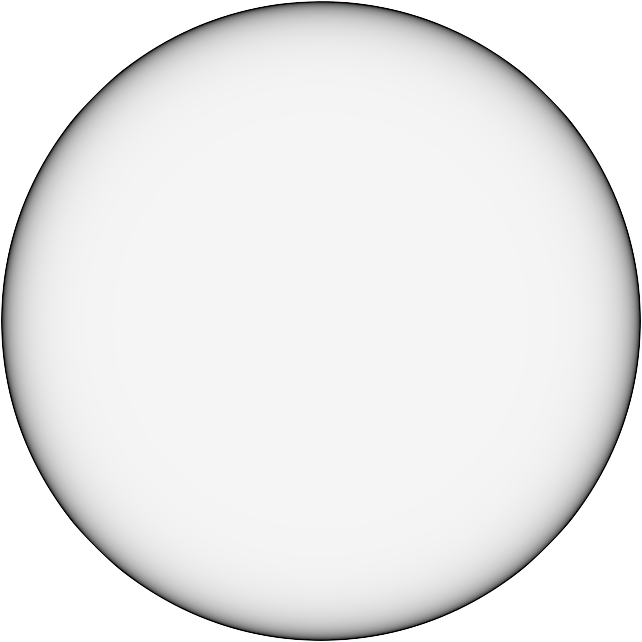
\includegraphics[width=5cm]{pbr/fresnel}
  \caption{Odwrócony współczynnik Fresnela, aproksymacja Schlicka}
\end{figure}

\subsection{Funkcja geometryczna}

Funkcja geometryczna (lub zaciemnianie geometryczne, ang. \textit{Geometric
Shadowing}) odpowiada za wspomniane wcześniej zjawiska rzucania cieni w obrębie
mikropowierzchni, w związku z czym światło które pada pod pewnym kątem nie
odbija się od całości powierzchni (ang. \textit{shadowing}, rys.
\ref{fig:GeometricShadowing}) oraz zasłaniania promieni odbitych od powierzchni
zmierzających do obserwatora przez inne elementy tej powierzchni w związku z
czym światło odbite nie dociera w całości do obserwatora (ang.
\textit{masking}). W realnym świecie promień po takim zderzeniu nie znika, ale
uproszczone modele traktują takie zachowanie jako absorpcję światła przez
powierzchnię.

Współczynnik związany z zaciemnianiem geometrycznym oznaczymy przez $G(l,v,h)$.
Wartość funkcji $G$ określa nam procent powierzchni skierowanych w kierunku
$h$, które nie są zaciemnione lub zasłonięte.

\begin{figure}[h]
  \centering
  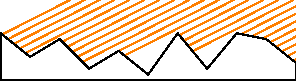
\includegraphics{illustrations/pbr/geometry_shadowing.pdf}
  \vspace{0.25cm}
  \caption{Samozacienianie wewnątrz mikropowierzchni}
  \label{fig:GeometricShadowing}
\end{figure}

Funkcja geometryczna nazywaną funkcją \textit{implicit} eliminującą czynnik
geometryczny definiujemy poprzez:
\[
  G_{\text{implicit}}(l,v,h) =
    (n \cdot l) (n \cdot v)
\]

\[
  G_{\text{Cook-Torrance}}(l,v,h) =
    \min \left(
      1,
      \frac{2(n \cdot h)(n \cdot v)}{
        v \cdot h
      },
      \frac{2(n \cdot h)(n \cdot l)}{
        v \cdot h
      }
    \right)
\]

Funkcje geometryczne korzystające z metody Smitha polegającej na rozbiciu
funkcji $G$ na dwa niezależne czynniki korzystające z tej samej funkcji $G_1$
z parametrem kolejno $l$ oraz $v$, tzn:
\[
  G(l,v,h) = G_1(l) G_1(v)
\]

% cite walter
Tak jak w poprzednim przypadku istnieje kilka modeli funkcji $G_1$.
Najpopularniejszymi wyborami są: GGX oraz aproksymacja Schlick-GGX:
\[
  G_{1}^{\text{GGX}}(v) =
    \chi^{+}\left(\frac{v \cdot m}{v \cdot n}\right)
    \frac{2}{
      1 + \sqrt{
        1 + \alpha^2 \tan^{2}\left(\theta_v\right)
      }
    }
\]
\[
  G_{1}^{\text{Schlick-GGX}}(v) =
    \frac{n \cdot v}{
      (n \cdot v)(1 - k) + k
    }
\]

gdzie $k = \frac{\alpha}{2}$.

\subsection{Podsumowanie}

Powyższe definicje umożliwają nam zbudowanie ogólnego modelu fizycznego
biorącego pod uwagę podstawowe zjawiska zachodzące w mikropowierzchniach
będących powierzchniami idealnie płaskimi.

W tej pracy będziemy korzystać głównie z funkcji rozkładu normalnych GGX,
aproksymacji Schlicka oraz funkcji geometrycznej GGX.

\todo[inline]{Dodać część diffuse Cook-Torrance}

\section{Swiatła punktowe}

Powszechną optymalizacją w grach komputerowych jest zastępowanie naturalnie występujących świateł powierzchniowych światłami punktowymi \cite{pbr_background}. Swiatła takie nie są fizycznie możliwe, lecz bardzo upraszczają obliczenia i w odpowiedniej skali potrafią bardzo dobrze aproksymować efekty świetlne nawet przy pominięciu powierzchni. Swiatla takie sa nieskończenie małe i jasne.

Podczas lokalnych obliczeń wpływu takiego światła parametrami będzie wektor łączący obecnie badany punkt na powierzchni $p$ oraz centrum światła $p_l$, którego znormalizowaną postać oznaczymy poprzez $l$ oraz kolor światła $\clightcolor$. Kolor światła $\clightcolor$ zdefiniujemy jako całkowitą odbitą radiancję dla 100\% białego materiału Lambertowskiego z normalną w kierunku zgodnym z kierunkiem wyznaczonym przez $l$, tzn:
\[
	\clightcolor = \frac{1}{\pi} \int_{\Omega} { L_i(\omega_l) (l \cdot \omega_i) \dd\omega_i }
\]

Załóżmy teraz, że w scenie występuje dokładnie jedno światło powierzchniowe o bardzo małej powierzchni. Całe światło jest zawarte w stożku o osi obrotowej leżącej na $l$ oraz o środku w punkcie $p$ o rozmiarze kątowym $\epsilon$. Dla pozostałych kierunków niezawartych w tym stożku radiancja jest zerowa. Przy założeniu, że $\clightcolor$ się nie zmienia oraz $\epsilon$ może być dowolnie mały otrzymujemy:
\[
	\clightcolor = \frac{1}{\pi} \lim_{\epsilon \rightarrow 0} \left(
		\int_{\Omega} { L_i(\omega_l) } \dd\omega_i
	\right)
	\Rightarrow
	\lim_{\epsilon \rightarrow 0} \left(\int_{\Omega} { L_i(\omega_l) } \dd\omega_i \right) = \pi\clightcolor
\]

Postępując analogicznie z równaniem renderingu otrzymujemy:
\[
	L_o(\omega_o) = \lim_{\epsilon \rightarrow 0} \left(
		\int_{\Omega}{ f(\omega_i, \omega_o) L_i(\omega_i) (n \cdot \omega_i) } \dd\omega_i
	\right) =
	 f(l, \omega_o) \lim_{\epsilon \rightarrow 0} \left(
	 	\int_{\Omega} { L_i(\omega_l) } \dd\omega_i
	 \right)
	 (n \cdot l)
\]

Podstawiając za całkę naszą stałą $\clightcolor$ finalnie otrzymujemy:
\[
	L_o(\omega_o) = \pi f(l, \omega_o) \clightcolor (n \cdot l)
\]

Jak widać, powyższe równanie aproksymuje obliczenie skomplikowanego wyrażenia całkowego jednokrotnym obliczeniem funkcji BRDF oraz kilkoma prostymi operacjami arytmetycznymi. Pozostaje pytanie, kiedy warto zastosować tego typu technikę. Aproksymacja ta, ma sens dla dynamicznych scen w których precyzja nie jest kluczowa oraz odleglość od źródła światła jest co namniej pięć razy większa od jego szerokości \cite{RealTimeRendering2008}\cite{lambert_photometria} - w takim przypadku konwersja na światło punktowe wraz z kwadratowym spadkiem intensywności powinna być wystarczająca w grach.


\section{Przybliżenie światła powierzchniowego klastrem świateł punktowych}

Pierwszą metodą, która nasuwa się po poznaniu podstaw jest podejśćie uproszczone polegające na przybliżeniu klasycznego światła powierzchniowego zbiorem świateł punktowych.

Będziemy badać światła powierzchniowe tego typu w formie prostokątnej ze względu na łatwość generowania jednorodnej siatki punktów wewnątrz takiego obszaru, kształt ten również posiada ostre krawędzie i rogi przez co minusy tej metody będą bardzo widoczne. Uogólnienie do dowolnego kształtu nie będzie wpływać na rezultaty jakościowo.

Załóżmy, że mamy prostokątne światło powierzchniowe o stałej irradiancji $E$ niezależnej od wybranego punktu. Wygenerujemy na nim siatkę jednakowych świateł punktowych z zastrzeżeniem, że działają one tylko gdy zachodzi warunek $n \cdot \omega_i > 0 $. To znaczy zakładamy, że światło powierzchniowe jest jednostronne.

Siatka punktowa będzie wygenerowana w taki sposób, aby każdy punkt przybliżał jednakowy fragment powierzchni światła (rys. \ref{fig:PointLightCluster}).

\begin{figure}[ht]
  \centering
  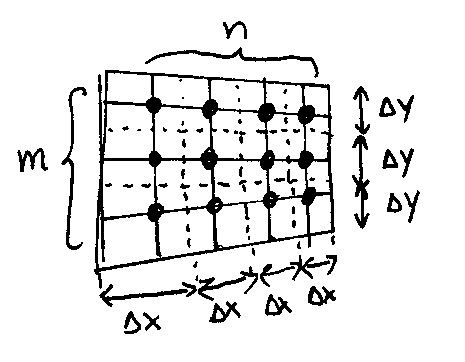
\includegraphics[height=5cm]{pbr/point_light_cluster.jpg}
  \caption{Klaster świateł punktowych na świetle powierzchniowym}
  \label{fig:PointLightCluster}
\end{figure}

Energia promieniowania dla tak zdefiniowanego przypadku można obliczyć korzystając z definicjii irradiancji:
\[
	\Phi = E \Delta{x} \Delta{y}
\]

Intensywność takiego źródła również będzie stała (dla danej długości fali $\lambda$) i równa: 

\[
  I 
	= \lim_{\Delta\omega \rightarrow 0} {
		\frac{\Delta\Phi}{\Delta\omega}
	} 
	= \frac{\Phi}{2\pi}
	= \frac{E\Delta{x}\Delta{y}}{2\pi}
\]

Korzystając z wcześniejszych definicji dla punktu $p$ na powierzchni i światła punktowego o środku w $l_c$ otrzymujemy \cite{pbr_frostbite}:
\[
	L_o(\omega_o) = \pi f(l, \omega_o) \frac{I}{r^2} (n \cdot l)
\]

\noindent gdzie $r$ jest równe $\norm{p-l_c}$.

Zatem dla całego klastra wystarczy zsumować wpływ każdego światła punktowego opisującego pewien podobszar:
\[
	L_o(\omega_o) = \pi \sum_{i}^{n} \sum_{j}^{m} {
		f(l_{i,j}, \omega_o) \frac{I}{(r_{i,j})^2} (n \cdot l_{i,j})
	}
\]

\end{document}
